%%%%%%%%%%%%%%%%%%%%%%%%%%%%%%%%%%%%%%%%%
% Short Sectioned Assignment
% LaTeX Template
% Version 1.0 (5/5/12)
%
% This template has been downloaded from:
% http://www.LaTeXTemplates.com
%
% Original author:
% Frits Wenneker (http://www.howtotex.com)
%
% License:
% CC BY-NC-SA 3.0 (http://creativecommons.org/licenses/by-nc-sa/3.0/)
%
%%%%%%%%%%%%%%%%%%%%%%%%%%%%%%%%%%%%%%%%%

%----------------------------------------------------------------------------------------
%	PACKAGES AND OTHER DOCUMENT CONFIGURATIONS
%----------------------------------------------------------------------------------------

\documentclass[paper=a4, fontsize=11pt]{scrartcl} % A4 paper and 11pt font size

\usepackage[T1]{fontenc} % Use 8-bit encoding that has 256 glyphs
\usepackage[ngerman]{babel}
\usepackage{fourier} % Use the Adobe Utopia font for the document - comment this line to return to the LaTeX default
\usepackage{amsmath,amsfonts,amsthm} % Math packages
\usepackage{graphicx}
\usepackage[utf8]{inputenc}
\usepackage{listings}
\usepackage[section]{placeins}
\usepackage{lipsum} % Used for inserting dummy 'Lorem ipsum' text into the template
\usepackage{float}
\usepackage{multicol}

\usepackage{sectsty} % Allows customizing section commands
\allsectionsfont{\centering \normalfont\scshape} % Make all sections centered, the default font and small caps

\usepackage{fancyhdr} % Custom headers and footers
\pagestyle{fancyplain} % Makes all pages in the document conform to the custom headers and footers
\fancyhead{} % No page header - if you want one, create it in the same way as the footers below
\fancyfoot[L]{} % Empty left footer
\fancyfoot[C]{} % Empty center footer
\fancyfoot[R]{\thepage} % Page numbering for right footer
\renewcommand{\headrulewidth}{0pt} % Remove header underlines
\renewcommand{\footrulewidth}{0pt} % Remove footer underlines
\setlength{\headheight}{13.6pt} % Customize the height of the header

\numberwithin{equation}{section} % Number equations within sections (i.e. 1.1, 1.2, 2.1, 2.2 instead of 1, 2, 3, 4)
\numberwithin{figure}{section} % Number figures within sections (i.e. 1.1, 1.2, 2.1, 2.2 instead of 1, 2, 3, 4)
\numberwithin{table}{section} % Number tables within sections (i.e. 1.1, 1.2, 2.1, 2.2 instead of 1, 2, 3, 4)

\setlength\parindent{0pt} % Removes all indentation from paragraphs - comment this line for an assignment with lots of text

\DeclareMathOperator*{\argmin}{arg\,min}

%----------------------------------------------------------------------------------------
%	TITLE SECTION
%----------------------------------------------------------------------------------------

\newcommand{\horrule}[1]{\rule{\linewidth}{#1}} % Create horizontal rule command with 1 argument of height

\title{	
\normalfont \normalsize 
\textsc{Karlsruhe Institute of Technology} \\ [25pt] % Your university, school and/or department name(s)
\horrule{0.5pt} \\[0.4cm] % Thin top horizontal rule
\huge Robotik 3 % The assignment title
\horrule{2pt} \\[0.5cm] % Thick bottom horizontal rule
}

\author{Manuel Lang} % Your name

\date{\normalsize\today} % Today's date or a custom date

\begin{document}

%\maketitle % Print the title
%\newpage
\tableofcontents
\newpage

\section{Sensoren}

\subsection{Definition}

\begin{itemize}
\item Sensoren sind Geräte, die physikalische Eigenschaften der Umgebung wahrnehmen und messen können (z.B. Temperatur, Helligkeit, Gewicht, Entfernung, etc.)
\item Sensoren liefern low-level Informationen über die anliegende Umwelt des Roboters. Diese sind limitiert, ungenau, verrauscht.
\item Also liefern Sensoren eine nicht komplette Beschreibung der Welt
\item Sensoren sind physikalische Geräte, die ein Signal oder einen Reiz empfangen und darauf mit einem elektrischen Signal reagieren
\item Jeder Sensor ist ein Energiewandler. Egal, was Sie messen, es geht immer um den Energietransfer vom Messobjekt zum Sensor.
\item Die Sensorik reicht von einfach bis komplex in der Informationsmenge.
\item Sensoren bilden das Wahrnehmungssystem eines Roboters
\item Sensoren ermöglichen das Schließen von Regelkreisen, die den effizienten und autonomen Betrieb von Robotern in der Praxis sicherstellen.
\end{itemize}

\subsection{Charakteristische Größen eines Sensors}

\begin{itemize}
\item Messbereich (range): [min, max]
\item Auflösung (resolution): kleinstes Inkrement eines Signals, das detektiert werden kann (Ein inkrementeller Encoder, der 1024 Impulse pro Umdrehung liefert hat eine Auflösung von $\frac{1 Umdrehung}{1024 Impulse} \cdot \frac{360 Grad}{1 Umdrehung} = 0.3516 \frac{Grad}{Impuls}$)
\item Empfinglichkeit (Sensitivity): Änderung des Ausgangs in Abhängigkeit von Änderung des Eingangs (Ein Sensor mit linearem Verhalten hat eine konstante Empfindlichkeit über den gesamten Messbereich)
\item Fehler (Error): Differenz zwischen gemessenem Wert und tatsächlichem Wert (Systematische Fehler - bias oder Genauigkeitsfehler)
\item Wiederholgenauigkeit (Repeatability): Fähigkeit identischen Output bei gleichem Input zu liefern
\item Linearität und Genauigkeit (Linearity und Accuracy): Genauigkeit $\sim$ Fehler eines Sensors (sehr genauer Sensor produziert sehr kleine Fehler), oft wird die Genauigkeit durch die Linearität ausgedrückt
\end{itemize}

\subsection{Klassifikation von Sensoren}

\begin{itemize}
\item Interne Sensoren: Erfassung innerer Zustände (z.B. Geschwindigkeitssensoren)
\item Externe Sensoren: Information über Zustand der Umwelt (z.B. Taktile Sensoren, Abstandssensoren)
\end{itemize}

\section{Interne Sensoren}

\subsection{Positionssensoren}

\subsubsection{Potentiometer}

\begin{minipage}{0.3\textwidth}
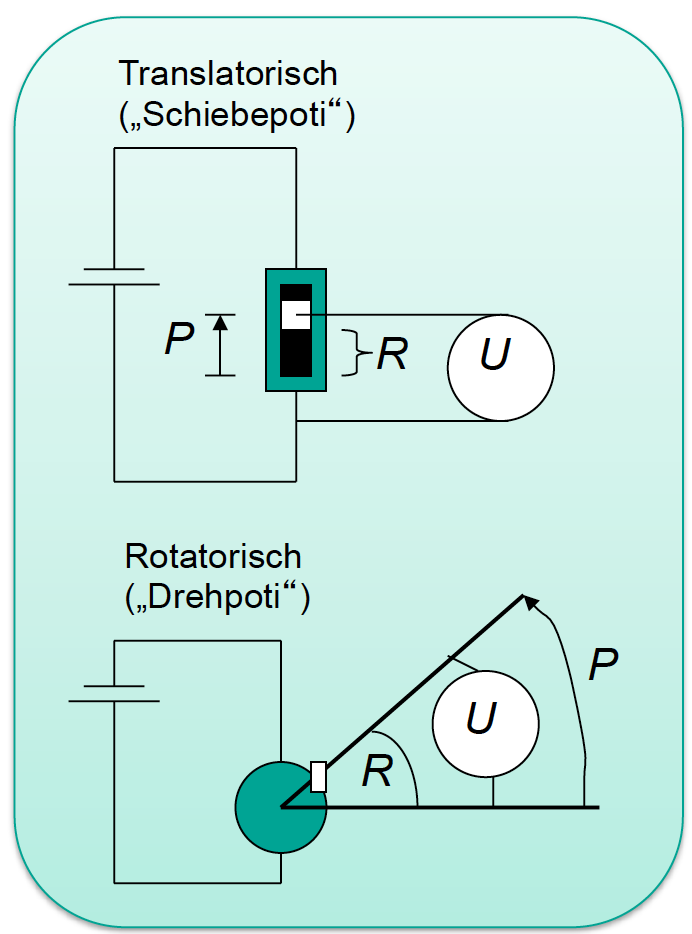
\includegraphics[width=\textwidth]{imgs/poti}
\end{minipage}
\begin{minipage}{0.6\textwidth}
\begin{itemize}
\item elektronisches Widerstandsbauelement, Widerstandswert mechanisch veränderbar, Spannungsteiler
\item lineare Position oder Drehposition
\item Messung der abgefallenen Spannung $U$ oder des Widerstands $U = \frac{R}{R_{ges}} * U_{ges}$ mit $R_{ges}$ als Gesamtwiderstand und $U_{ges}$ als Gesamtspannung
\item Widerstand proportional zur Position $P$ -> $R \sim P$ -> $U \sim P$
\end{itemize}
\end{minipage}

\subsubsection{Optische Codierer}

\begin{itemize}
\item Information über Position von rotatorischen oder translatorischen Gelenken oder über die relative Position eines Fahrzeuges
\item Inkrementelle optische Codierer
\begin{itemize}
\item Lichtstrahl wird auf Photodetektor ausgerichtet, auf einer Schreibe angebrachtes codiertes Muster (Code) unterbricht periodisch den Strahl (Schreibe mit durchsichtigen und undurchsichtigen Stellen)
\item Unterbrechungen werden gemessen und evtl. der Code festgestellt
\item Vorteile: einfache Kodierscheiben, einfache Zählung
\item Startposition unbekannt (Kalibrierung notwending)
\item 1-spurige Codierscheibe (Winkel): Anzahl der Impulse $\sim$ gefahrener Winkel, bei kontrollierter Fahrt: ok, bei Störeinfluss: Richtung der Störung? -> Regelung nicht möglich aber für Steuerung geeignet
\item 2-spurige Codierscheibe (Winkel und Richtung): versetzte Dioden bzw. Codes (Phasenverschiebung gewöhnlich 90°/270° zwischen Diodensignalen, Richtung aus Phasenverschiebung, Regelung möglich), Problem: Initialisierung/Wiederanfahren (Position unbekannt?) -> Kalibrierung notwending, aber nicht unmöglich
\item 3-spurige Codierschreibe (Winkel, Richtung, Anfang/Ende): zusätzlich Anfang/Ende-Markierung, kontrolliertes Fahren in Initialposition (falls 1 Umdrehung genügt), Initialisierung der Regelgrößen
\item Problem: bei Stromausfall gehen alle Positionssensoren verloren, so dass eine Kalibrierung nach jedem Systemstart notwendig ist
\end{itemize}
\item Absolute optische Codierer
\begin{itemize}
\item Position absolut codiert, d.h. jederzeit bekannt, keine Initialisierung
\item Statt serielle Bitströme (inkrementellen Sensoren) werden parallele Wortsignale mit einem Wortmuster (Code) für jede Achsenposition geliefert
\item Vorteile: diskretes Ablesen der Gelenkposition, kein Datenverlust durch Stromausfall
\item Nachteil: aufwendiger Aufbau
\item Unterschied zum inkrementellen Codierer: jede quantifizierte Achsposition enthält ein individuelles Wortmuster (-> Gray-Code ist fehlertoleranter als Binärcode)
\end{itemize}
\end{itemize}

\subsection{Geschwindigkeitssensoren}

\begin{itemize}
\item Gleichstromtachogenerator
\begin{itemize}
\item Ausgangsspannung $V_0$
\item Winkelgeschwindigkeit $\omega_s$
\item $V_0 = K_t \cdot \omega_s$
\item Arbeitsprinzip: elektromagnetische Induktion (Faradays Gesetz)
\item Ausgangsspannung in großen Bereichen proportional zu Geschwindigkeit
\end{itemize}
\item Wechselstromtachogenerator: Gleichrichtung erforderlich
\item Tachometer auf Basis eines optischen Codierers: Frequenz der gemessenen Impulse proportional zu Geschwindigkeit
\end{itemize}

\subsection{Beschleunigungssensoren}

\begin{itemize}
\item Beschleunigung ist nur durch Wirkung auf träge Masse messbar
\item Anwendungen: Airbag, Neigungsmessung, Vibrationsmessung, Stabilisierung von Flugzeugen, ...
\item Messprinzipien
\begin{itemize}
\item Wegmessung an Feder-Masse-System: häufigstes Messprinzip, Ausschlagverfahren -> Messung des Federwegs (ausgelöst durch Masseträgheit), Kompensationsverfahren -> Messung der Kraft zum Halten der Feder in Mittellage/Nulllage
\item Geschwindigkeitsmessung an viskos gedämpfter Masse: gut geeignet für Stoßmessungen wegen Überlastsicherheit
\item Weg-Zeit-Messung bei frei schwebenden Körpern: geeignet für sehr hohe Auflösungen z.B. Messungen an Satelliten (über Zeit hinweg wird immer wieder zurückgelegter Weg gemessen)
\end{itemize}
\item Damped spring-mass system: $x = K(g-x)-Dx$ mit goal attractor - damping term
\end{itemize}

\subsubsection{Piezoresistiv}

\begin{itemize}
\item Messprinzip: Seismische Masse
\item Mikrosystemtechnik: Ätzen einer trägen Messe und deren Aufhängungen in Silizium (Auslenkung ändert mechanische Spannungen, welche den piezoresistiven Widerstandswert ändern, Wiederstandswert mechanisch erfassbar)
\item Anwendung in der Robotik: Auslenkung zur Erdanziehung oder Lage im Raum
\end{itemize}

\subsubsection{Piezoelektronisch}

\begin{itemize}
\item Messprinzip: Seismische Masse (Testmasse mit definiertem Wert)
\item Werkstoff PXE mit piezoelektrischen Eigenschaften
\item Piezokeramischer Wandler verbindet freischwingende Masse M mit Aufnehmerboden
\item Beschleunigung wirkt als Kraft über der Masse M
\item Ausgangsspannung abhängig von Beschleunigung
\item Piezoelektrischer Effekt: wird ein piezoelektrisches Material mechanisch belastet, treten durch Verformung der Elementarzellen an dessen Oberfläche elektrische Ladungen auf.
\item Umwandlung in proportionale Spannung über integrierten Verstärker/Elektrometerverstärker 
\end{itemize}

\subsection{Inertial Navigation System (INS)}

Lagesensoren
\begin{itemize}
\item beziehen sich immer auf inertiales Koordinatensystem (zumeist auf Erdkugel)
\item Kompass: Magnetometer, Kreiselkompass
\item Gravitometer: Messeung des Erdschwerefeldes -> Neigungssensor
\end{itemize}

\subsubsection{Gyroskop (Kreiselkompass)}

\begin{itemize}
\item Kreisel, kardanisch aufgehängt, schnell drehend
\item Aufgrund des Drehimpulserhaltungssatzes behält er seine Orientierung im Raum bei -> Drehwinkel zwischen Kreisel und Käfig messbar
\end{itemize}

\subsubsection{Mikromechanische Vibrationskreisel}

\begin{itemize}
\item Mikromechanische Drehratensensoren beruhen auf Resonanzstrukturen und Energieübertragung zwischen den genutzten Schwingmoden (Primär- und Sekundärmode) durch dir Coriolisbeschleunigung -> Foucault-Pendel
\item Antriebsprinzipien: elektrostatisch, elektromagnetisch, piezoelektrisch
\item Messprinzipien: kapazitiv, piezoresistiv, piezoelektrisch
\end{itemize}

\section{Externe Sensoren}

\subsection{Taktile Sensoren}

\begin{itemize}
\item Umweltinformationen durch direktes Berühren von Objekten (physikalischer Kontakt zwischen Roboter und Werkstück)
\item Einsatz: Ermittlung geometrischer Größen (Lage, Orientierung, Form), Ermittlung physikalischer Größen (Kräfte, Momente, Druck), einfachste Berühungssensoren: Mikroschalter (binäre Aussage über Kontakt)
\item Dehnungsmessstreifen: verformt sich bei Krafteinwirkung, Veränderung des ohmschen Widerstands, Problem: Dehnungsempfindlichkeit von Leitern gering, Lösung: Messsignal erhöhen durch mäanderförmige Struktur
\item Piezoeletrische Sensoren: Vorteile: unempfindlich gegenüber hohen Temperaturen (bis 1000°C), keine äußere Spannungsversorgung notwendig, hoher Wirkungsgrad der Umwandlung von mechanischer in elektrische Energie, geringe mechanische Eigenschwingung und Hysterne durch starren Aufbau
\item Force Sensing Resistor (FSR)
\begin{itemize}
\item Folienschalter, halbquantitative Sensoren
\item Aufbau: FSR-Schicht (Trägerschicht mit halbleitendem Polymer), elastische Klebeschicht als Abstandshalter, Elektrodenschicht (kammförmige Trägerfolie mit Elektroden)
\item Bei Druck berührt FSR-Schicht die Elektrodenschicht, es bilden sich Widerstandsbrücken
\item Widerstandsänderung abhängig von Kraft (exponentiell)
\item Vorteile: preiswert, dünn, sehr haltbar, widerstandsfähig
\item Nachteil: nicht hochgenau
\item Messbereich: 10g bis 10.000g
\end{itemize}
\item Drucksensitive Materialien: Verkürzung von oder Entstehung neuer Strompfade bei Belastung (z.B. Elastomer mit Kohlenstoffbeimischung), Verstärkung des Effekts durch Schicht, die aus teilweise leitfhähigem Silikon besteht, das durch Abstandshalter von einer leitfähigen Leiterplatte getrennt wird
\end{itemize}

\subsubsection{Tastende \& gleitende Sensoren}

\begin{itemize}
\item Magnetoelastischer Sensor: magnetisch isotropes Material wird unter Druck anisotrop (Aufbau: 2 zueinander orthogonale Spulen in ferromagnetischem Material)
\item Magnetoresistiver Sensor: Änderung des spezifischen Widerstands unter Einfluss eines veränderlichen Magnetfeldes (Aufbau: Ni-Fe-Element, stromführender Leiter, Gummi)
\item Hallsensor: Wirkung eines magnetischen Feldes auf stromdurchflossenen Halbleiter -> Umwandlung der Druckkraft in Wegänderung und Ausgangsspannung
\item Taktil gleitende Sensoren: Information über Oberflächenbeschaffenheit und geometrische Struktur
\end{itemize}

\subsubsection{Kraft-Momenten-Sensoren}

\begin{itemize}
\item Erfassung der Kräfte zwischen Effektor und Handhabungsobjekt
\item aktiv: Feststellen ausgeübter Kräfte/Momente (Sicherheit/Genauigkeit)
\item passiv: Führen des Roboters durch den Benutzer (Teach-In/Interaktion)
\end{itemize}

\subsection{Näherungssensoren}

\begin{itemize}
\item erkennen Objekte in gewisser Reichweite vom Roboter
\item liefern binäres Signal
\item kontaktfreie Geräte die für Hinderniserkennung verwendet werden
\end{itemize}

\subsubsection{Optische Sensoren}

\begin{itemize}
\item basieren auf Lichtreflektion
\item Lichtschwelle: binäre Ausgabe
\item Vorteile: größere Entfernungen, kontaktfrei, einstellbarer Schwellwert
\item Reflektion von Licht (Rotlicht-LED)
\item Laufzeit-/Triangulationsmessung
\item Standard in Automation, sehr teuer
\end{itemize}

\subsubsection{Akkustische Sensoren}

\begin{itemize}
\item Verschicken Ultraschallwellen (20-200 KHz) und messen Reflektion anhand von Energieänderung
\item Vorteile: Emission und Detektion mit gleichem Converter, sehr hohe Reichweite
\item Rauschen
\end{itemize}

\subsection{Abstandssensoren}

\begin{itemize}
\item Messung der Distanz zwischen Sensor und Objekt
\item Vorteile: größere Reichweite als Näherungssensoren, extakte Distanz als Ausgabe statt binärem Wert, anwendbar zur Erkennung von geometrischen Informationen über die Umwelt
\item aktive Abstandssensoren: Verwendung einer Lichtquelle zur Beleuchtung der Umwelt (Laser scanner, TOF Kamera, Laserstreifen, Musterprojektion)
\item passive Abstandssensoren: benötigen keine Lichtquelle -> verwenden Umgebungslicht (Stereo-Kamera-Systeme)
\end{itemize}

\subsubsection{Laufzeitbasiert}

\begin{itemize}
\item messen die benötigte Zeit eines Laserimpulses vom Emitter zum Objekt und zurück
\item Distanz berechnet sich mit $d = \frac{1}{2} ct$ mit Ausbreitungsgeschwindigkeit $c$ und der messbaren Zeit $t$, der Faktor 0.5 um die Entfernung in eine Richtung zu bestimmen
\item erreicht mittels Radar, Sonar, Lichtwellen
\item Mögliche Fehlerquellen: Variationen in der Ausbreitungsgeschwindigkeit (z.B. bei Temperaturunterschieden), Unsicherheiten bei der Zeitbestimmung, Interaktion zwischen Schallwelle und Objektoberfläche
\end{itemize}

\subsubsection{Triangulationsbasiert}

\begin{itemize}
\item In einem Stereo-Kamera-System wird eine der Kameras mit einer aktiven Lichtquelle versehen
\item Projiziere den Laserstrahl in die Szene und nehme in mit einem positionssensitiven Sensor auf
\item Vereinfachung des Korrespondenzproblems
\end{itemize}

\subsection{Visuelle Sensoren}

\begin{itemize}
\item Anwendungen: Mobile Robotik, Humanoide Robotik, Industrie-Robotik, Sicherheitssysteme, Qualitätskontrolle, Objekterkennung ...
\item Probleme: Kamerabewegung, unscharfe Kamerabilder, Objekterkennung nicht erfolgreich 
\item Lösungsansätze: Gaze Stabilization, Active Vision
\end{itemize}

\subsubsection{Photodioden}

\begin{itemize}
\item Innerer Photoeffekt (Halbleiter in eine Richtung durchlässig, bei Licht wird Halbleiter durchlässig und Strom fließt -> Photonenenergie) -> verwendet in Photodiode, CCD, CMOS
\item Rückschluss von Strom auf Licht (ca. linear)
\item Aufbau: Laserstrahl, Halbleiter mit 2 Elektroden, konstante Spannung, Lichtstrahl auf Diode -> Position des Lichtstrahls bestimmbar
\item Quadranten-Photodiode: 2-dimensionale Bestimmung des Lichtstrahls (z.B. CD-Spieler, Blue-ray-player)
\end{itemize}

\subsubsection{CCD (Charge coupled devices, unterschiedliche Übertragungstechniken)}

\begin{itemize}
\item Analoger Speicherbaustein, Prinzip Eimerkette (linke Seite Ladung -> Transport durch Anlegen von Spannung)
\item Bild zeilenweise nach unten vorschoben und horizontal ausgelesen
\item Bestandteile: Photodioden und elektronische Schaltung (Lichtstärke analog in digitales Bild, Clock/Taktgeber, Vorschaltung (Gain) - höheres Rauschverhältnis, umgewandelt in digitales Signal liefert digitales Bild)
\item CCD als Framesensor (nach unten verschoben - horizontales Ausgaberegister) -> Problem: Belichtung während Auslesen (Bild verschmiert -> Shutter), große Sensorfläche, einfach, Anwendung in der Astronomie
\item doppelte Sensorfläche, untere Hälfte z.B. lichtunempflindlich mit z.B. Aluminiumüberzug -> Nachteil: doppelter Platz aber kein Shutter nötig, schnell, einfach
\item Interline-Transfer-Sensor: jeder 2. Sensor ist mit Alu-Schicht lichtumempfindlich, Ladung nach links -> unten -> ... Vorteil: sehr kurze Belichtungszeiten, elektronischer Shutter, Nachteil: doppelte Sensorfläche, größerer Füllfaktor, lichtempfindliche und lichtunempfindliche Zellen nah beieinander -> Einsatz von Lisen über Sensorzellen, damit Licht an ungenutzer Sensorzelle eingefangen werden kann -> höherer Dynamikumfang, Sensoren empfindlicher, zusätzliche Linsen nötig (sehr kleine Linsen)
\item Interline-Transfer: Auslesen streifenförmiger Anordnung, 2 Pixel zusammen + 4-Phasen-Zellen-Schieberegister + Anlegen von Spannung -> Verschiebung der aufgefassenen Lichtimpulsen
\item Betriebsarten: Field- vs Frame-Integration: Zeileneinweise Auslesen
\item Interlaced: erst gerade Zeilen, dann ungerade Zeilen, Bilder als Habbild übertragen (gerade Zeilen und ungerade Zeilen)
\item Non-Interlaced: nicht mehr nötig heutzutage
\item Field Integrations Interlaced: Speicherzellen mit örtlichem Zeitversatz auslesen, Takt getrennt, elektronischer Shutter kann verwendet werden (zusätzliches Löschen nötig -> besseres Bild)
\item Frame Integration Interlaced: versetzte Beleuchtung ergibt zeitlichen Überlappungsbereich, bei dem analoges Signal ausgelesen wird
\item Progressive: Vorteil der Halbbilder fällt weg, Zellen nacheinander ausgelesen, teilweise parallelisierbar
\item Blooming-Effekt: starke Lichtquelle strahlt auf Nachbarpixel über (örtlich begrenzt)
\item Verschmiereffekt bei Full-Frame-Sensor: während Auslesen wird Sensorfläche belichtet erzeugt Streifen im Bild
\end{itemize}


\subsubsection{CMOS (Frontkamera Smartphone, Complementary Mental Oxide Semiconductor)}
\begin{itemize}
\item Ladungs-/Spannungskonvertierung pro Pixel bringt digitales Signal (CCD nur analog)
\item Vorteil: einzelnes Ansprechen der Pixel möglich -> Auflösung reduzieren und größerere Daten übertragen, Windowing einfach realisierbar
\item Nachteile: Ladungs-/Spannungskonvertierung nötig, wenig Bauteilfläche, Fehler: Rolling Shutter: zeitliche Verschiebung bei Beleuchtung der Pixel -> Lösung: zusätzliche Transistoren bei Pixeln -> Global Shutter\\ 
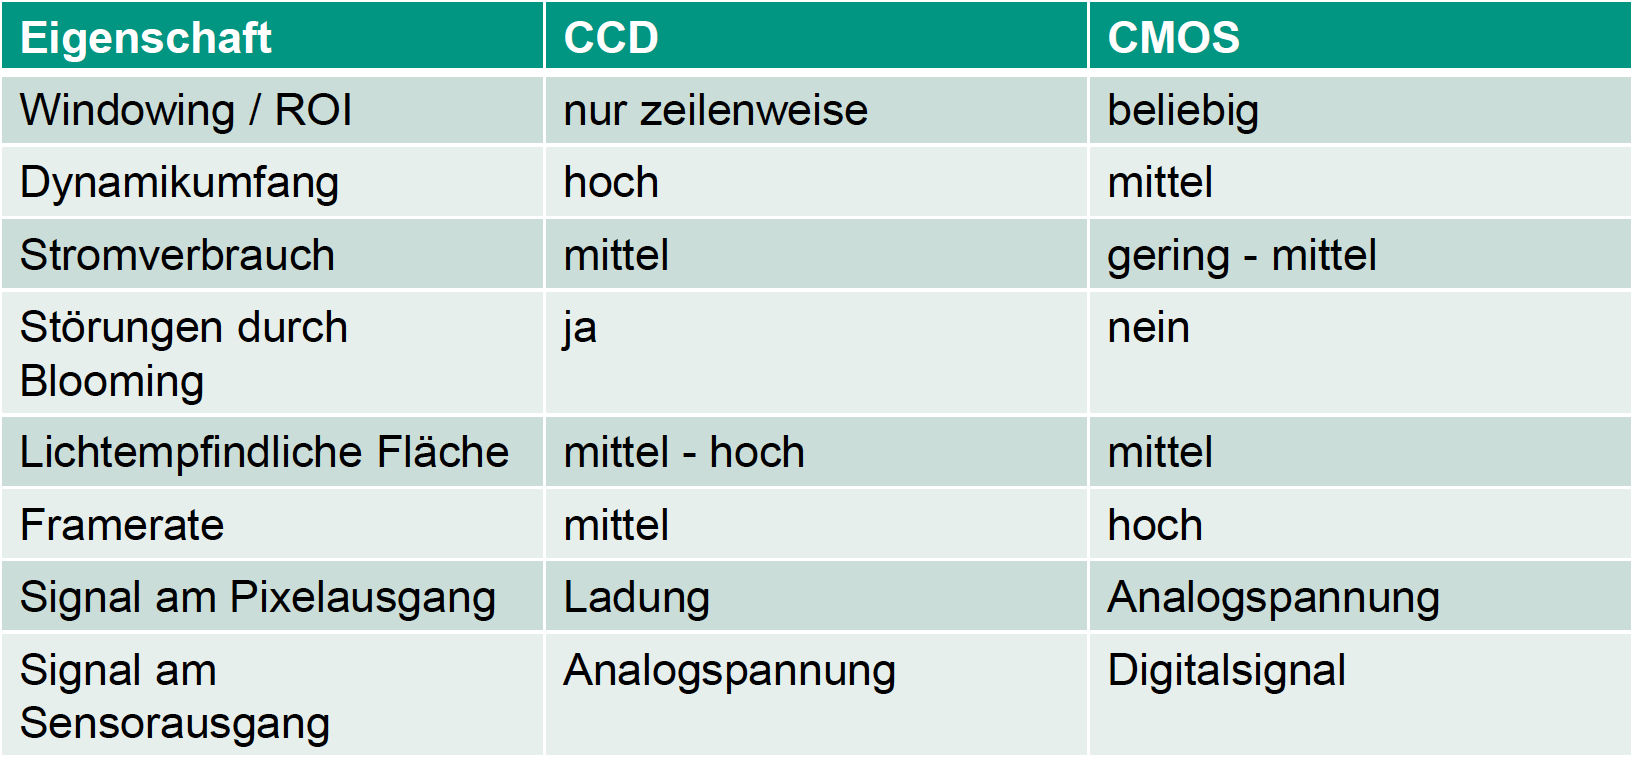
\includegraphics[width=\textwidth]{imgs/ccd_cmos}
\item CCD sehr zuverlässig, Trend zu CMOS
\end{itemize}

\subsubsection{Farbverarbeitung}
\begin{itemize}
\item 3-Chip-Methode: Prisma davor, Licht trennen mit unterschiedlichen Wellenlängen (RGB), Vorteil: hohe Auflösung, Schärfe, Nachteil 3 Sensoren, teures Prisma
\item 1-Chip-Methode (Bayer-Pattern): Pixel in unterschiedliche Farben aufgeteilt (RGB) -> Filtermaske in unterschiedliche Wellenlängen, jeder Pixel liefert andere Farbinformation, nicht so globig, Bandbreite kann eingesparrt werden
\end{itemize}

\subsubsection{Kamerasysteme}

\begin{itemize}
\item Bildaufnehmer-Formate
\begin{itemize}
\item Zoll Format: alt, bezog sich auf Röhrentechnik, Vidiconschlauch mit Außendurchmesser von 1 Zoll besaß ein rechteckiges, lichtempfindliches Fenster mit einer Diagonalen von 16mm (1/3", 1/2", 1/1.8", 2/3", 1", 4/3")
\item APS Format: folgt dem ``Advanced Photo System'', wenn Bild-Sensoren das Format 4/3" übersteigen wird der APS Formatstandard verwendet
\end{itemize}
\item Objektive
\begin{itemize}
\item C-/CS-Mount: normiertes Objektivanschlussgewinde
\item Objektive haben i.d.R. einstellbaren Fokus
\item Brennweite fest oder variabel (Zoom)
\item Blende: Blendenzahl beschreibt relative Öffnung der Blende, preiswerte Objekte besitzen u.U. keine Blende
\item Mini-Objektive (keine Blende, fester Fokus, feste Brennweite, sehr klein, sehr günstig)
\end{itemize}
\item Analog- und Digitalkamera
\begin{itemize}
\item Analogkameras: ausschließlich CCD, kein CMOS, Spannungen am Sensorausgang des CCD-Chips werden seriell übertragen, Anschluss über Frame-Grabber-Karte an den PC, Frame-Grabber führt A/D-Wandlung durch
\item Digitalkameras: Anschluss über Firewire, USB, Camera Link, Ethernet, liefern direkt digitalisierte Bilddaten
\end{itemize}
\end{itemize}

\subsubsection{Bildrepräsentation}

\begin{itemize}
\item Bild ist 2D Gitter von diskreten Punkten (Pixeln)
\item Farbe eines Bildpunktes kann auf unterschiedliche Weise repräsentiert werden
\item Graustufenbilder: Helligkeitswert [0,255] für jeden Pixel
\item Farbbild: verschiedene Farbmodelle für unterschiedliche Anwendungen, Klassifikation nach erreichbarem Farbraum (z.B. RGB/HSV)
\item RGB zu Grau: menschliches Auge ist am empfindlichsten gegenüber der Farbe grün -> $g = 0.299 \cdot R + 0.587 \cdot G + 0.114 \cdot B$
\end{itemize}

\subsection{Positionssensoren}

\begin{itemize}
\item Grundlage: aktive beacons
\item Anwendung: Navigation von Schiffen, Flugzeugen, Fahrzeugen
\end{itemize}

\subsubsection{Global Positioning System (GPS)}

\begin{minipage}{0.3\textwidth}
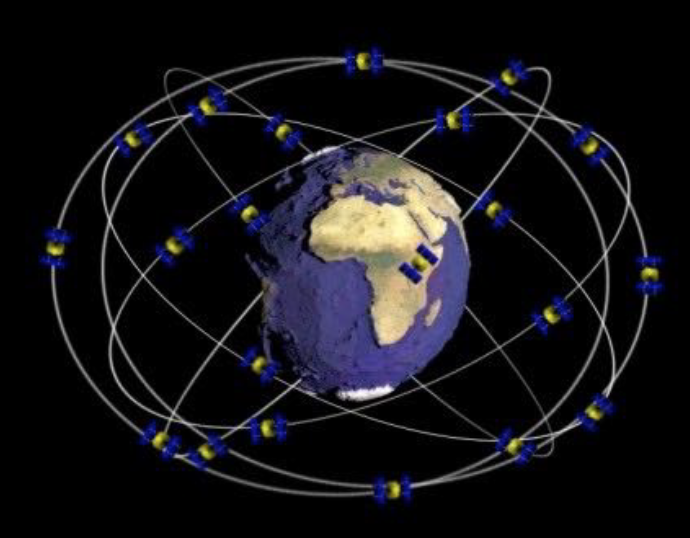
\includegraphics[width=\textwidth]{imgs/gps}
\end{minipage}
\begin{minipage}{0.6\textwidth}
\begin{itemize}
\item Satellitengestütztes Navigations- und Punktbestimmungssystem, 24 Satelliten, Umlaufzeit 12 Stunden, Entfernung 20051 Kilometer, 6 Bahnebenen
\item Bedingung: mindestens 4 Satelliten in Reichweise
\item Messung: Codephase (Pseudoentfernung), Doppler-Count (Geschwindigkeitsmessung), Trägermischphase (Messung der Strecke mittels Phasenverschiebung)
\item Aufgaben der Master-Control-Station: Vorausberechnung Bahnephemeriden, Beobachtung Satellitenuhren, Vorausberechnung Satellitenverhalten, Weitergabe von Daten
\end{itemize}
\end{minipage}

\subsubsection{Natürliche/künstliche Landmarken}

\begin{itemize}
\item nicht aktiv
\item einfach zu identifizieren
\item feste und bekannte Position
\item Problem: Detektion, Matchen
\item künstliche Landmarken: speziell auf Umgebung abgestimmt
\end{itemize}

\section{Sensormodellierung}

\begin{itemize}
\item Zusammenhang zwischen realer Welt und Messergebnis
\item Sensormodell: mathematische Beschreibung der Aufnahmecharakteristik eines Sensors\\ 
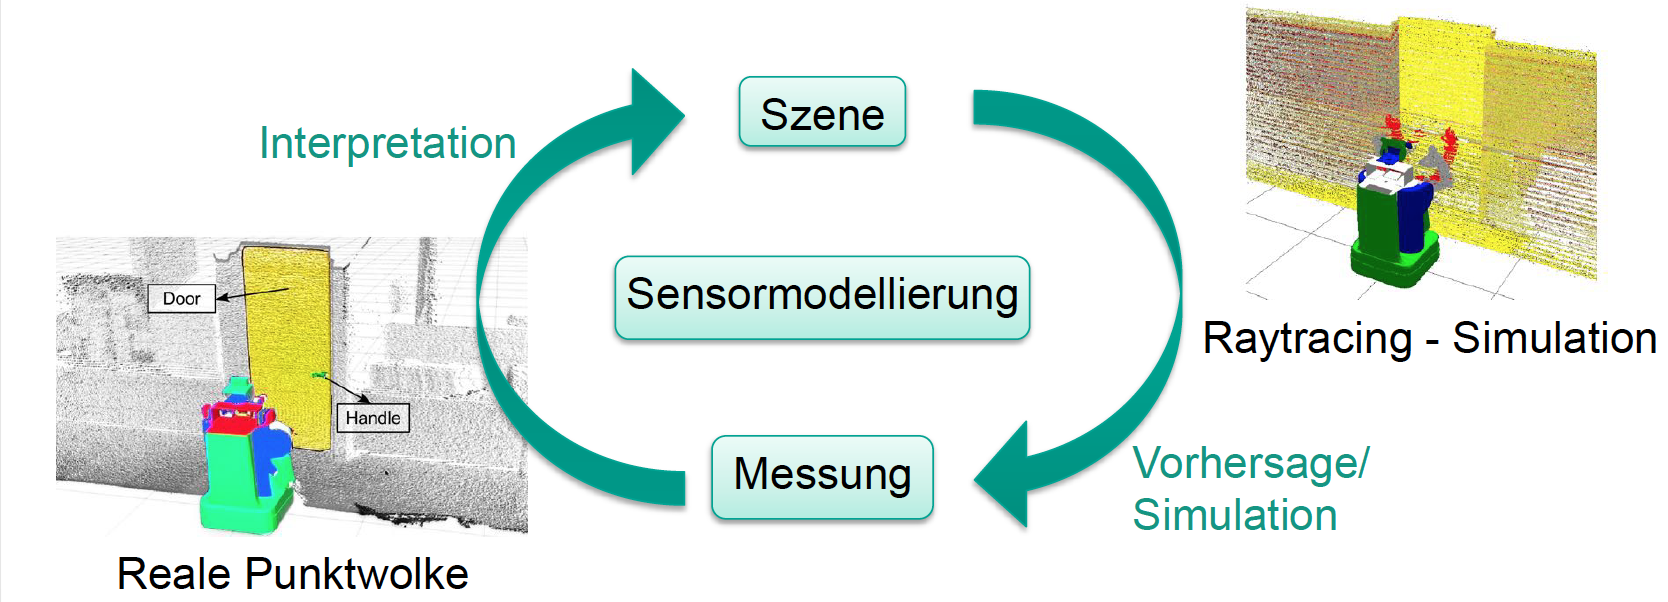
\includegraphics[width=\textwidth]{imgs/sensormodellierung}
\item Aufgaben
\begin{itemize}
\item Interpretation von Messaten (Reale Aufnahme -> (Sensormodell)$^{-1}$ -> Szenenbeschreibung)
\item Vorhersage von Messdaten (Szenenbeschreibung -> Sensormodell -> Aufnahmewerterwartung)
\item Sensorsimulation (Szenenbeschreibung -> Sensormodell -> Fehlermodell/Rauschen -> Messergebnis)
\end{itemize}
\item jeder Sensormesswert ist fehlerbehaftet, aber Fehler lässt sich mathematisch modellieren
\item setzt sich zusammen aus systematischem Fehler und Restfehler
\item Kalibrierung behebt systematischen Fehler
\item Robuste Algorithmen beheben Restfehler
\end{itemize}

\subsection{Mathematischen Sensormodell}

\begin{itemize}
\item Abbildung des Umweltzustands in den Bildraum $z_m(\Theta_n) + v_m$ mit Beobachtungsmodell $h$, normalverteiltem Rauschen $v_m$ und Umweltzustand $\Theta_n$
\item $h$ hängt vom Sensortyp (KMS, Datenhandschuh, Kamera) und von festen spezifischen Parametern (Position der Kamera im Raum) ab
\item Feste Kalibrierungsparameter charakterisieren Übertragungseigenschaften eines Sensors
\item Dynamische Sensorparameter, auch Steuerparemeter genannt, beschreiben veränderliche Eigenschaften eines Sensors.
\end{itemize}

\subsection{Modellierung}

\subsubsection{Kraft-Momenten-Messdose}

\begin{itemize}
\item Prinzip: Kräfte/Momente -> Deformation des Dehnungsmessstreifens -> Änderung des Widerstands, Spannungsabfall
\item Näherung: Linearer Zusammenhang Kraft <-> Spannung
\item N-Sensorelemente $W = c_{i1} F_x + c_{i2} F_y + c_{i3} F_z + c_{i4} M_x + c_{i5} M_y + c_{i6} M_z$ mit $W_i$: Spannung an Sensor i, $F_x$: Kraftkomponente, $M_x$: Momentenkomponente und $c_{ij}$: Koppelfaktoren
\item Kalibrierung $C$ gesucht: Messung der $W$ bei bekannten Kräften $F$, Aufstellen eines (überbestimmten) LGS für $C$, Lösung des LGS nach $C$ (kleinste Quadrate) mit pseudoinverser Matrix $R_F$ der Kopplungsmatrix
\end{itemize}

\subsubsection{Datenhandschuh}

\begin{itemize}
\item 22 Sensorelemente (DMS) mit jeweils affinem Modell: $W_i = c_i \cdot \alpha_i + t_i$
\item 22 DMS werden getrennt kalibriert, Daten jedoch simultan erhoben
\item Griffe von Kalibrierobjekt liefern für alle i Gelenkwinkel jeweils n Messungen
\item Bestimmung der Parameter aus überbestimmten LGS
\end{itemize}

\subsubsection{Modellierung einer Kamera}

\begin{itemize}
\item Modellierung der Lichtintensität abhängig von Beleuchtung der Szene und Reflexionseigenschaften der Objekte
\item Modellierung der Geometrie: dreidimensionale Szene wird abgebildet auf zweidimensionale Fläche
\end{itemize}

\subsubsection{RotatingSick}

\begin{itemize}
\item besteht aus SICK LMS 200 Laserscanner
\item über Drehdurchführung an Dunker-Motor-Kombination gekoppelt
\item Prinzip des LMS 200: Ausstrahlung - Modul. Signal -> Reflextion an Objekt -> Empfang - Phasenverschobenes Signal
\item Entfernung des Reflexionsobjekts: $d = \frac{1}{2} c \cdot t$
\end{itemize}

\subsection{Sensorsimulation}

\begin{itemize}
\item mit gutem Modell können Sensoren simuliert werden
\item Nutzen: Prädiktion (verbessert Ungenauigkeiten durch Fusionierung mit zusätzlichem virtuellen Messwert, kann Ausreißer erkennen), Simulation (Ausprobieren ohne Hardwareaufwand)
\item Deterministisches Modell kann nie vollständig Sensor simulieren (Messung immer fehlerbehaftet, größter Simulationsaufwand: korrekte Fehlerstimulation)
\item Sensor-Aufnahmefähigkeit: Welche Merkmale unter welchen Bedingungen?
\item Sensor-Zuverlässigkeit: Maß für die Unsicherheiten der Messung (Beitrag des Rauschens zur Messung eines Merkmals)
\end{itemize}

Gross Error Model
\begin{itemize}
\item Annahme hier: Messungen verhalten sich in der Regel normalverteilt, in seltenen Fällen aber falsche Messungen nach Modell $n_g$ -> Wahrscheinlichkeitsdichte für $n(u)$:\\ $p(u) = \frac{1-\epsilon}{(2\pi) det(A_1))^{m/2}}e^{-\frac{1}{2}(u-\tilde{u})^T A_1^{-1}(u-\tilde{u})} + \frac{\epsilon}{(2\pi det(A_2))^{m/2}} e^{-\frac{1}{2}(u-\tilde{u})^T A_2^{-1}(u-\tilde{u})}$
\item Annahmen: Kovarianzmatrix $A_1$ bekannt, $0.01 << \epsilon << 0.05$, $det(A_1) << det(A_2)$
\end{itemize}

\section{Signalverarbeitung}

\begin{itemize}
\item Sensor: Ein System, das eine physikalische Größe und deren Änderung in geeignete elektrische Signale umwandelt
\item Digitale Signalverarbeitung (analog -> digital): Signalerfassung -> Aufbereitung (Verstärkung) -> Digitalisierung
\item Signal: physikalische Repräsentation von Information, meist physikalische Größe als Funktion von Zeit und/oder Ort
\item Analoges Signal: Amplitude kann kontinuierlich jeden Wert zwischen und Minimum und Maximum annehmen -> wert- und zeitkontinuierlich, i.d.R. Spannungssignale
\item Digitales Signal: Wertebereich und Zeit/Ort diskret (erlauben komplexere Signalumformungen für Sprach- und Bildverarbeitung)
\item Signalverstärkung: Ausgangsgröße des Sensors (i.d.R. Spannung/Strom) verstärken
\end{itemize}

\subsection{Digitalisierung}

\begin{itemize}
\item Verarbeitungsschritte: Abstatung/Rasterung (Amplitudenmessung zu diskreten Zeitpunkten), Quantisierung (Abbildung des kontinuierlichen Wertebereichs auf diskreten Wertebereich)
\item Analog/Digitalwandlung: Bereich des analgen Signals wird in $2^n$ gleichgroße Abschnitte eingeteilt, liegt ein Spannungswert in einem der durch Digitalisierung erzeugten Teilabschnitte vor, so ordnet man ihm den Digitalwert der unteren Abschnittsgrenze zu, Schaltungen zum Realisieren einer A/D-Wandlung: Dual-Slope-Wandler, Sukzessiver Approximationswandler, FlashWandler/Parallelwandler
\end{itemize}

\subsection{Fourier-Transformation}

\begin{itemize}
\item Digitale Signalverarbeitung: Umformung von Zahlenfolgen aus Abtastung analoger Signale
\item transformiert die Darstellung einer Eingabefunktion zwischen Ortsraum und Frequenzraum
\item von Ortsraum zu Frequenzraum: Berechnung der Anteile periodischer Strukturen in der Eingabefunktion (Projektion der Eingabe auf sin() und cos() für verschiedene Frequenzen)
\end{itemize}

\subsection{Abtasttheorem}

\begin{itemize}
\item Rekonstruierbarkeitsproblem (Abtastwerte -> kontrinuierliches Signal)
\item Notwendige Abtastfrequenz nach Shannonschem Abtasttheorem: Abtastfrequenz > doppelte maximale Signalfrequenz
\item bei geringerer Abtastfrequenz: Aliasing-Effekt
\end{itemize}

\section{Optische 3D Sensoren}

\subsection{Lochkameramodell}

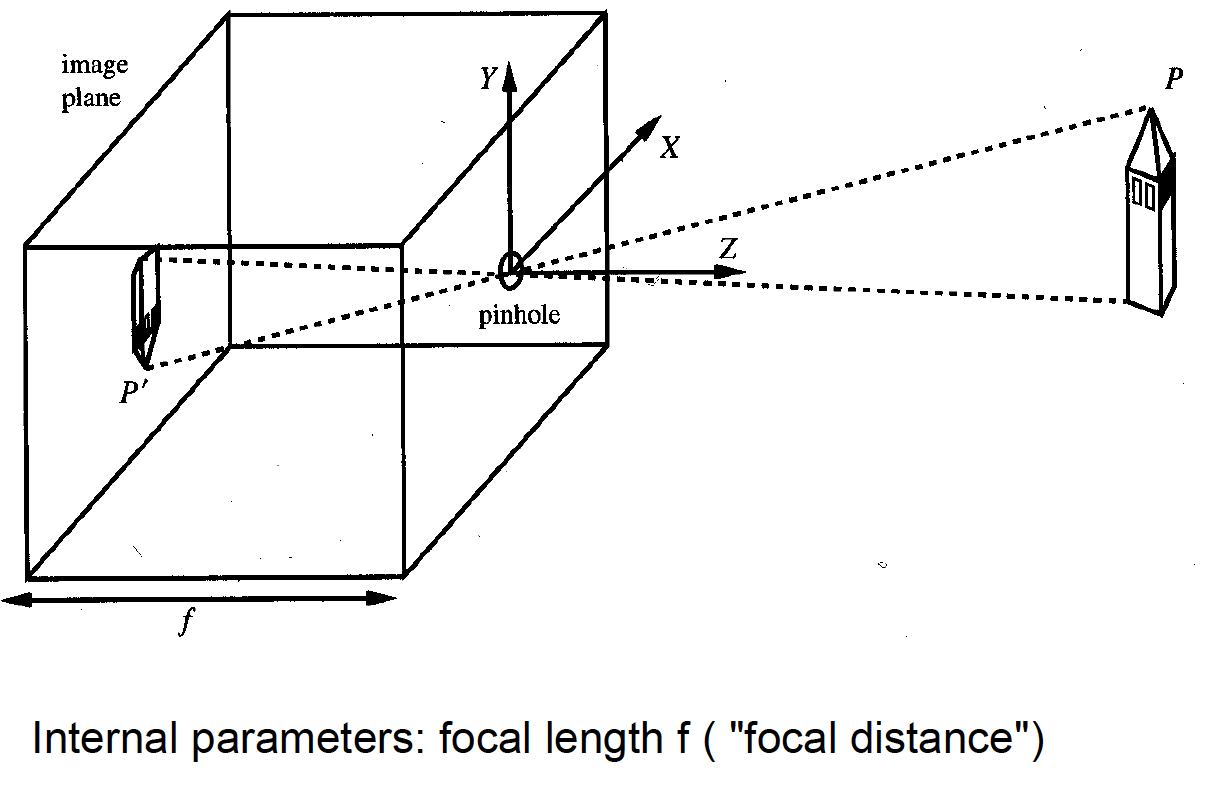
\includegraphics[width=\textwidth]{imgs/lochkamera}

Projektion eines Szenenpunkts $P = (X,Y,Z)$ auf einen Pixel $P = (u,v,w)$:

$-\frac{u}{f} = \frac{x}{z}, -\frac{v}{f} = \frac{y}{z}, w = -f$

$p = \begin{pmatrix} u \\ v \\ w \end{pmatrix} = \begin{pmatrix} u \\ v \\ -f \end{pmatrix} = -\frac{f}{z} \begin{pmatrix} x \\ y \\ z \end{pmatrix} = -\frac{f}{z} P$

Rückprojektion: $x = -\frac{uz}{f}, y = -\frac{vz}{f}$

\subsection{Erweitertes Kameramodell}

\begin{itemize}
\item Lochkameramodell vereinfacht stark, praktisch nicht realisierbar -> Anpassung
\item Optische Achse: geht durch Projektionszentrum, senkrecht zur Bildebene
\item Principal point $C$: Schnittpunkt der optischen Achse mit Bildebene
\item Koordinatensysteme
\begin{itemize}
\item Bildkoordinatensystem: 2D Koordinatensystem mit der Einheit [pixel], Ursprung (0,0) links/oben, u- und v-Achse
\item Kamerakoordinatensystem: 3D Koordinatensystem mit der Einheit [mm], Ursprung im Zentrum der Projektion, Achsen parallel zu denen des Bildes (+ 3-Finger-Regel)
\item Weltkoordinatensystem: 3D Koordinatensystem mit der Einheit [mm], beliebig im Raum
\end{itemize}
\item Parameter
\begin{itemize}
\item intrinsisch: Brennweite, Bildpunkt, Parameter zur Beschreibung der Linsenverzerrung, definieren Beziehung zwischen Kamerakoordinaten und Bildkoordinaten
\item extrinsisch: definieren Beziehung zwischen Kamerakoordinaten und Weltkoordinaten durch eine Rotation $R$ und eine Translation $T$
\end{itemize}
\item Vereinfachungen des Lochkameramodells: Principle point ist in der Mitte der Bildebene, Pixels sind quadratisch, keine Modellierung der Linsenverzerrung, kein Weltkoordinatensystem (oder gleich wie Kamerakoordinatensystem) -> keine extrinsischen Parameter
\item Die Bildkoordinaten sind dann bestimmbar durch: $\begin{pmatrix} u \\ v\end{pmatrix} = \begin{pmatrix} c_x \\ c_y\end{pmatrix} + \frac{1}{Z} \begin{pmatrix} f_x \cdot X \\ f_y \cdot Y\end{pmatrix}$\\ oder als Matrixmultiplikation mit der Kalibrierungsmatrix $K$ in homogenen Koordinaten: $\begin{pmatrix} u \cdot w \\ v \cdot w \\ w\end{pmatrix} = K \begin{pmatrix} X \\ Y \\ Z\end{pmatrix}$ mit $K = \begin{pmatrix} f_x & 0 & c_x \\ 0 & f_y & c_y \\ 0 & 0 & 1\end{pmatrix}$
\item Extrinsische Kamerakalibrierung
\begin{itemize}
\item definiert durch durch eine Koordinatentransformation mit Rotation $R$ und Translation $T$
\item Koordinatentransformation vom Weltkoordinatensystem ins Kamerakoordinatensystem: $x_c = Rx_w + t$
\item Ergebnis ist eine 3x4 Projektionsmatrix $P$ (mit intrinsischen und extrinsischen Parametern) in homogenen Koordinaten: $\begin{pmatrix} u \cdot w \\ v \cdot w \\ w\end{pmatrix} = P \begin{pmatrix} X \\ Y \\ Z \\ 1\end{pmatrix}$, $P = (KR|Kt)$
\end{itemize}
\item Linsenverzerrung: Bildgebung bei realen Linsen ist nicht perfekt linear, Linsen mit kurzer Brennweite bilden Verzerrung
\item Kamerakalibrierung: Bestimmung der Parameter bezüglich eines Kameramodells, Bestimmung der intrinsischen Parameter ist unabhängig von der Struktur, Bestimmung der extrinsischen Parameter abhängig vom Weltkoordinatensystem
\end{itemize}

\subsection{Stereogeometrie/Epipolargeometrie}

\begin{itemize}
\item Stereo-Rekonstruktion: mit 2 Kameras und 2 Bildern eines Punktes, kann dieser Punkt rekonstruiert werden
\item Epipolargeometrie beschreibt die Verbindung zwischen 2 Kameras
\item Epipolarlinien definieren alle Schnittpunkte der Epipolarebene mit der Bildebene
\item Fundamentalmatrix ist eine mathematische Beschreibung der Epipolargeometrie, 3x3 mit Rang 2
\item Korrespondenzproblem lösbar durch
\begin{itemize}
\item Time coded methods / Temporal Coding: viele (binär codierte) Streifen werden nacheinander projiziert
\item Phase shift method: Sinusförmige Grauwerte werden auf die Szene projiziert
\item Frequency encoding: Coding über Farbe (RGB -> HSV (verwende V-Wert))
\end{itemize}
\end{itemize}

\section{Bildverarbeitung}

\subsection{Histogramme}

\begin{itemize}
\item Wie bildet man ein Histogramm? -> Zählen der Farb-/Grauwerte
\item normalisiertes Histogramm -> Teilen durch Anzahl an auftretenden Werten liefert Wahrscheinlichkeit
\item Histogrammausgleich: bilde akkumuliertes Histogramm und berechne $\frac{255}{N} H_a(x)$ (für Grauwerte)
\end{itemize}

\subsection{Filter}

\subsection{Glättung - Tiefpass}

\begin{itemize}
\item Median-Filter: verwende Median von Nachbarschaft
\item Mittelwert-Filter: $ \frac{1}{9} \begin{pmatrix} 1 & 1 & 1\\ 1 & 1 & 1\\ 1 & 1 & 1 \end{pmatrix}$
\item Gauß-Filter: $ \frac{1}{16} \begin{pmatrix} 1 & 2 & 1\\ 2 & 4 & 2\\ 1 & 2 & 1 \end{pmatrix}$
\end{itemize}

\subsection{Kantendetektoren - Hochpass}

\begin{itemize}
\item Prewitt: z.B. $p_x = \begin{pmatrix} -1 & 0 & 1\\ -1 & 0 & 1\\ -1 & 0 &1\end{pmatrix}$
\item Prewitt-Operator: $M = \sqrt{P_x^2 + P_y^2}$
\item Sobel: z.B. $s_y = \begin{pmatrix} -1 & -2 & -1\\ 0 & 0 & 0\\ 1 & 2 & 1\end{pmatrix}$
\item Laplace: entweder $\begin{pmatrix} 0 & 1 & 0\\ 1 & -4 & 1\\ 0 & 1 & 0\end{pmatrix}$ (invariant ggü. Rotation in 90°) oder  $\begin{pmatrix} 1 & 1 & 1\\ 1 & -8 & 1\\ 1 & 1 & 1\end{pmatrix}$ (invariant ggü. Rotation in 45°)
\item Laplacian of Gaussian: $LoG(g(x,y)) = \nabla^2(f(x,y) * g(x,y))$
\item Canny Edge Detector
\begin{enumerate}
\item Glättung: Gauss
\item Kantendetektion in x- und y-Richtung (Prewitt/Sobel)
\item Non-Maximum Suppression
\item Hysteresis thresholding
\end{enumerate}
\end{itemize}

\subsection{Segmentierung}

\begin{itemize}
\item Aufteilung des Bildinhalts in sinnvolle Elemente (z.B. Vordergrund/Hintergrund)
\item Schwellwert auf Graubild
\item Region Growing (angrenzende Pixel: $|Img(p_0) - Img(q)| \le \epsilon$)
\item Segmentierung mit Farbwerten z.B. für Hautfarbe (HS-Histogramm)
\item Hough Transformation ($r = x cos \theta + y sin \theta$) liefert Repräsentation der geometrischen Struktur
\end{itemize}

\section{Merkmalsextraktion}

\subsection{Korrelationsfunktionen}

\begin{itemize}
\item Sum of Squared Differences (SSD): pixelweise Unterschiede quadriert und aufsummiert
\item Sum of Absolute Differences (SAD): pixelweise Unterschiede aufsummiert (weniger anfällig ggü. Ausreißern)
\item weitere Ansätze: ZSAD (Subtraktion des Mittelwerts), NSSD (Division durch die Frobeniusform), ZNSSD(Kombination beider)
\end{itemize}

\subsection{Eckendetektoren}

\subsubsection{Moravec-Operator}

\begin{itemize}
\item Ziel: Ähnliche Bereiche in aufeinanderfolgenden Kamerabildern wiederfinden
\item Konzept der Punktmerkmal (Interest Points)
\item Punktmerkmal wird als ein Punkt definiert, von dem aus sich die Intensität in alle Richtungen stark verändert
\item Nutzen von Autokorrelationsfunktion
\item Vorgehen: Verschiebe quadatrisches Fenster in 4 Richtungen (horizontal, vertikal, beide Diagonalen) und berechne jeweils SSD -> geringer Wert: (nahezu) homogener Bereich, Wert ist für Verschiebung längs einer bestimmten Richtung R aus S gering, für Verschiebungen senkrecht zu R jedoch hoch -> Kante entlang R, D überall hoch -> Ecke (Punktmerkmal)
\item Nachteile: Anisotropische Antwort des Operators (nicht invariant gegenüber beliebigen Rotationen), verrauschte Antwort des Operators (Pixel in den Ecken können wegen quadratischem/binären Aufbau das Ergebnis verfälschen), starke Antwort bei Kanten (Operator findet Ecken bei Kanten, die nicht exakt entlang der vordefinierten Verschiebungsrichtungen laufen)
\end{itemize}

\subsubsection{Harris Corner Detector}

\begin{itemize}
\item Ziel: Ersetzung der vier vordefinierten Richtungen durch ein Verfahren, welches eine feinere Schrittweite erlaubt
\item Ausgangsbasis ist Taylorentwicklung erster Ordnung (Richtungsableitungen benötigt -> Prewitt oder Sobel)
\item Approximation von Autokorrelationsfunktion durch quadratische Form über Matrix M (d.h. Gradienten)
\item M enthält Information über die Struktur des Bildbereichs (Ellipse konstanter Grauwertänderung)
\item Struktur lässt sich aus Eigenwerten von M ableiten
\begin{enumerate}
\item beide Eigenwerte klein -> große Ellipse -> (nahezu) homogener Bereich
\item ein EW groß, der andere klein -> gestreckte Ellipse -> Kante
\item beide EW groß -> kleine Ellipse -> Ecke (Punktmerkmal)
\item Zusammenfassung der EW in Concerness $C(u,v) = m_{11} m_{22} - m_{12} m_{21} - \kappa(m_{11}+m_{22})^2$
\end{enumerate}
\end{itemize}

\subsubsection{Good Features To Track}

\begin{itemize}
\item Verbesserte Fassung des Harris Corner Detektors durch explizite Berechnung der Eigenwerte der Matrix $M(u,v)$
\item Bedingung für Merkmale: $min(\lambda_1,\lambda_2) > \lambda$ (Schwellwert) statt Concerness
\end{itemize}

\subsection{Einfache Deskriptoren}

\begin{itemize}
\item Einfachster Ansatz: Beschreibung der lokalen Umgebung durch ein Quadrat um den zu betrachtenden Bildpunkt (Bildausschnitt als Merkmal), Vergleich zweier Ausschnitte durch Anwendung einer Korrelationsfunktion
\item Vorteile: einfach zu realisieren, geringer Rechenaufwand
\item Nachteil: keine Invarianz bzgl. Rotation und Skalierung
\item Erweiterung nach Lepetit
\begin{itemize}
\item Modellierung jedes Bildausschnitts durch ein sog. view set
\item Generierung von z.B. 100 Ansichten des lokalen Ausschnitts welche den Raum der möglichen Erscheinungen abdecken (Skalierung, Rotation, Verzerrung)
\item Abgleich (Matching) eines Bildausschnitts aus der aktuellen Szene mit der Datenbank durch Vergleich mit allen Ansichten aller eingelernten Bildausschnitte
\item Ansichten können synthesisch generiert werden durch Verzerrungsabbildung (affine Transformation, texturiertes 3D-Modell und Rendering)
\item Nachteil: hoher Speicher- und Rechenaufwand
\item Lösungsansatz: PCA -> Reduktion von 1024 auf 20 Dimensionen beschleunigt und reduziert Speicheraufwand
\end{itemize}
\end{itemize}

\subsection{Aktuelle Merkmale (Detektor + Deskriptor)}

\subsubsection{Scale Invariant Feature Transform (SIFT)}

\begin{itemize}
\item Generieren verschiedener Bildauflösung äquivalent zu sukzessivem Gaußglätten und Unterabtasten (sonst: Aliasing)
\item Detektor arbeitet auf der Basis einer Skalenraum-Analyse mit Difference of Gaussians (DoG)
\item Deskriptor besteht aus in Teil-Quadrate unterteiltem Gradientenhistogramm
\item Verfahren ist invariant bzgl. Rotation und in einem kleinen Bereich bzgl. Verzerrung
\item Merkmalsdetektor
\begin{itemize}
\item Skalenraum wird aufgebaut durch Faltung mit der Gauß-Funktion
\item Stabile Merkmalspunkte werden durch Bestimmung von Extrema der DoG-Funktion berechnet
\item DoG-Funktion ist eine effiziente Approximation des skalennormalisierten LoG-Operatos, der ein Blob Detektor ist. LoG erkennt Blob nur bei passender Skalierung
\end{itemize}
\item Deskriptor
\begin{itemize}
\item Tiefpass-gefiltertes Bild entsprechend der Skala, auf welcher der Keypoint detektiert wurde, wird für die Berechnung der Deskriptors verwendet
\item Berechnung der Gradienten in einem quadratischen Fenster (gewichtet mit Gauß-Funktion)
\item Berechnung des Betrags und der Richtung
\item Berechnung eines Gradientenhistogramms mit 10° Diskretisierung (36 Bins) über $\theta$ und $m$ als Gewichtung
\item Berechnung des globalen Maximums. Ausgabe dessen und aller Einträge mit Werten $\ge 85\%$ des Maximums sind Richtungen
\item Für jede der berechneten Richtungen wird das Bild rotativ entsprechend der Richtung ausgerichtet (Rotationsinvarianz) und ein Deskriptor berechnet
\end{itemize}
\end{itemize}

\subsubsection{Speeded Up Robust Features (SURF)}

\begin{itemize}
\item Motivation: Geschwindigkeitssteigerung gegenüber SIFT bei vergleichbaren oder verbesserten Eigenschaften
\item Ansatz: Verwendung von Rechtecksfiltern (beschleunigte Berechnung durch Integral Images) anstatt DoG, Deskriptor um Faktor 2 kleiner: 64 Dimensionen
\end{itemize}

\subsubsection{Maximally Stable Extremal Regions (MSER)}

\begin{itemize}
\item Idee: stabile, homogene Regionen (mit kontrastierendem Rand) detektieren, ohne Vorgabe eines Schwellwerts
\item Ansatz: Analyse der Folge aller durch Schwellwertfilterung berechneter Binärbilder, Finden von Bildregionen, die über hohe Anzahl von Schwellwerten ihre Form \& Ausdehnung nicht ändern
\end{itemize}

\subsection{Matching von Merkmalen}

\begin{itemize}
\item Vergleich der Merkmalsvektoren mit entsprechendem Fehler- bzw. Korrelationsmaß
\item Nearest-Neighbor
\item k-Nearest-Neighbor
\item Matching-Strategien
\begin{itemize}
\item zu jedem Merkmal im Anfrage-Bild ordne ein entsprechendes Merkmal aus der Datenbank zu
\item zu jedem Merkmal aus der Datenbank ordne ein ensprechendes Merkmal aus dem Anfrage-Bild zu
\item oder Kombination der beiden o.g. Strategien
\end{itemize}
\end{itemize}

\subsection{Objekterkennung auf der Basis von Punktmerkmalen}

\begin{itemize}
\item Bag of Features
\begin{itemize}
\item Zählen der Korrespondenzen für eine gegebene Objektrepräsentation bestehend aus einer Menge von Punktmerkmalen
\item Zuordnung erfolgt ausschließlich auf der Basis der Merkmalsvektoren
\item Objekt gilt als erkannt, wenn eine erforderliche Mindestanzahl an Korrespondenzen berechnet wurde
\item Vorteil: einfach zu realisieren
\item Nachteil: nicht robust, fehleranfällig
\end{itemize}
\item RANSAC
\begin{itemize}
\item iteratives Verfahren, um eine bezüglich eines gegebenen Modells konsistente Untermenge einer Menge robust zu bestimmen
\item Haupteinsatzzweck: Filtern von Ausreißern
\end{itemize}
\item Least Squares
\begin{itemize}
\item Anwendng für die Berechnung einer Homographie bzw. Affintransformation
\item Gegeben: Menge von Punktkorrespondenzen
\item LGS lösen zur Bestimmung von Homographie/Affintransformationen
\end{itemize}
\end{itemize}

\subsection{6-DoF Lageschätzung}

\begin{itemize}
\item Bestimmung der 3D-Transformation welche die 6-DoG Lage des Objektkordinatensystems (gegebenes 3D-Modell) im Weltkoordinatensystem beschreibt
\item Monokulare Lageschätzung 
\begin{itemize}
\item 2D-3D Punktkorrespondenzen (3D-Punkte des Modells und 2D-Punkte aus der aktuellen Ansicht (Bildkoordinaten))
\item Korrespondenzen müssen beim Einlernen für das Trainingsbild bzw. die Trainingsbilder bestimmt werden
\item Über die bei der Erkennung berechnete Homography können die 2D-3D Punktkorrespondenzen propagiert werden oder Propagation durch Tracking der 2D-Punkte
\end{itemize}
\item Stereo-basierte Lageschätzung
\begin{itemize}
\item Eine Möglichkeit: Berechnung von 3D-Koordinaten für Merkmalspunkte über Korrelation und Stereo-Triangulation, anschließend: Fitting eines geometrischen 3D-Primitivs, Registrierung eines 3D-Objektmodells
\item Vorteile: robust aufgrund von Stereo-Triangulation, je nach Aufbau höhere Genauigkeit
\item Nachteile: Ungenauigkeiten bei starken Linsenverzerrungen
\end{itemize}
\end{itemize}

\section{Umweltmodellierung}

\begin{itemize}
\item Roboter benötigt Weltmodell, das die reale Welt auf innere Repräsentation abbildet (Information über Umweltbeschaffenheit, Sammlung von räumlichen Beziehungen)
\item Notwendige Informationen zur Aufgabenbewältigung: Navigation, Positionsbestimmung, Sensordatenverarbeitung
\end{itemize}

\subsection{Abstraktionsniveau: Sensordaten <-> Semantik}

\begin{itemize}
\item Geometrische Darstellung: Anwendung in Bahnplanung (feinkörnig), aktives Mesen, Objekterkennung, Fahren von $P_1$ nach $P_2$
\item Topologische Darstellung: Anwendung in Planung (Manipulationsplanung, mittlere Körnigkeit, Bahnplanung, ``Fahre von Raum 1 nach Raum 5'')
\item Semantische Darstellung: Anwendung in Planung auf Aufgabenebene, ``Fahre durch alle Büros''
\end{itemize}

\subsection{Operationsraum des Roboters: 2D <-> 3D}
\begin{itemize}
\item 2-dimensional: Anwendung in Bahnplanung mobiler Roboter, Werkstückanalyse, 2D-Bearbeitung
\item 2.5-dimensional: Anwendung bei Approximation unbekannter Objekte, niedrigere Komplexität als 3D, einfache 3D-Welten -> Bahnplanung einfach
\item 3D-Szene: komplexere Umweltmodellierung, realistische Modellierung, komplexe Sensorik, komplexe Planung
\end{itemize}

\subsection{Umweltbedingungen des Roboters: Statisch <-> Dynamisch}
\begin{itemize}
\item Statisch: bekannte Umwelt -> alle Objekte in Weltmodell vorhanden, selten reale Anwendung
\item Dynamisch: unbekannte Umwelt -> Umweltinformationen durch Kartografierung, Berücksichtung der Positionsänderung von Objekten
\end{itemize}

\subsection{Anwendungsgebiet des Roboters: Strukturiert <-> Unstrukturiert}
\begin{itemize}
\item Strukturiert: wenige verschiedene Objekte, gut wahrnehmbare Bewergungsgrenzen \& Fahrflächen, meist in geschlossenen Räumen
\item Unstrukturiert: häufig im freien Gelände, wichtige Fehlerquellen: unebener, rutschiger Untergrund, fehlende Landmarke
\end{itemize}

\subsection{Informationsgehalt}
\subsubsection{Pfade} 
\begin{minipage}{0.6\textwidth}
\begin{itemize}
\item normal 2 bis 2.5-dimensionaler Raum
\item polygonale Beschreibung der Objekte
\item Pfad: lineare oder nichtlineare Verbindung zweier Punkte im Operationsraum
\item Speicherung der Umwelt- und Planungsinformationen
\item Repräsentation als ungerichteter Graph
\item einfache Umweltdarstellung, partielle Modellierung
\item kollisionsfreie Bewegung nur auf gespeicherten Pfaden
\item Sichtbarkeitsgraphen zur automatischen Generierung von Pfaden
\end{itemize}
\end{minipage}
\begin{minipage}{0.3\textwidth}
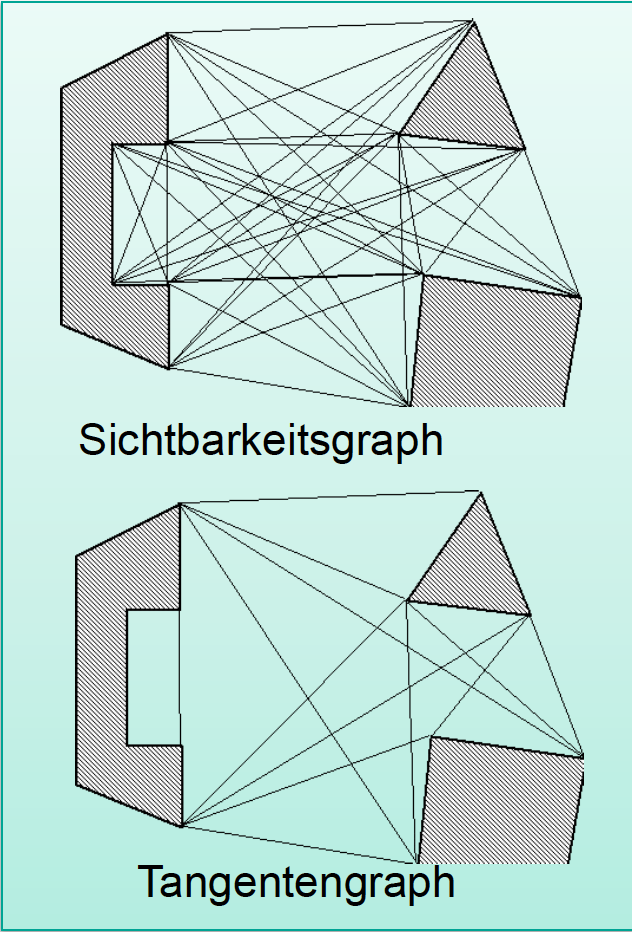
\includegraphics[width=\textwidth]{imgs/sichtgraph}
\end{minipage}
\subsubsection{Freiraum}
\begin{minipage}{0.6\textwidth}
\begin{itemize}
\item Projektion der realen Welt in 2-dimensionale Grundrissdarstellung
\item Kollisionsfreie befahrbare Freiräume in geeignete Bereiche zerlegt
\item Vorhandene Objekte und Hindernisse nicht berücksichtigt
\end{itemize}
\end{minipage}
\begin{minipage}{0.3\textwidth}
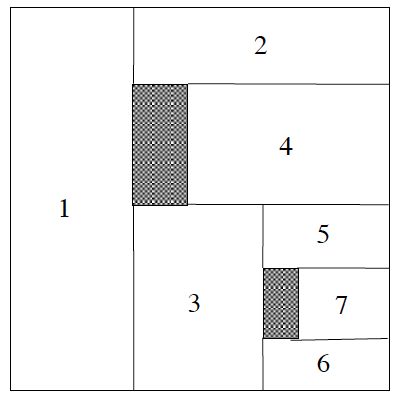
\includegraphics[width=\textwidth]{imgs/freiraum}
\end{minipage}
\subsubsection{Objekte}
\begin{itemize}
\item Darstellung der Objekte der realen Umwelt (Türen, Wände, Hindernisse)
\item 3-dimensionale Darstellung der Umgebung aus Sensorwahrnehmung
\item Projektion auf x-y-Ebene für Navigation bodengebundener Roboter ausreichend
\item Verschiedene Darstellungen
\begin{itemize}
\item Kantenmodelle: Ermittlung von markanten Punkten, Verbinden durch geeignete Kanten auf Oberfläche des Objekts
\item Oberflächenmodelle: Nachbildung der Objektoberflächen, Darstellung ebener Flächenelemente mit Polygonen, gekrümmte Flächenelemente: mathematisch beschreibbar (Zylinder, Kegel, Torusfläche), näherungsweise durch Freiformflächen (patches)
\item Volumenmodelle: Unterscheidung von Raumpunkten hinsichtlich ihrer Lage zum Objekt (innen- außenliegend), verschiedene Repräsentationsmöglichkeiten
\begin{itemize}
\item Begrenzungsflächenmethode: Beschreibung des Körpers durch umgebende geometrische Elemente (Flächen, Kanten, Punkte)
\item Grundkörperdarstellung: Zusammensetzung von Körpern aus parametrierbaren Grundelementen (die bekannt oder gespeichert sein müssen)
\item Cell Decomposition: Zusammensetzung aus Einzelelementen -> Zerlegung komplizierter Körper in einfache Teile
\item Volumenapproximation: Objektbeschreibung durch Würfel
\item Einhüllende Quader: Objektbeshreibung durch Quader unterschiedlicher Größe, Geradensegmente: Erkennung bzw. Generierung von Geradensegmenten (Parametrische Umweltdarstellung aus Sensormessungen, Zusammenfassen von Messwerten zu Regionen konstanter Entfernung, Darstellung als Geradensegmente, Erkennung von zylindrischen Hindernissen, konvexen und konkaven Ecken
\end{itemize}
\end{itemize}
\end{itemize}
\subsubsection{Gemischte Modelle}
\begin{itemize}
\item In der Forschung am häufigsten eingesetzt
\item Unterschied zu bisherigen Modellen: Erfassung von Freiräumen und Objekten
\item Wichtigste Methoden
\begin{itemize}
\item Gitter- bzw. Rasterdarstellungen
\begin{itemize}
\item Zwei bzw. dreidimensionale Rasterstruktur
\item Annäherung der Form des Hindernisses durch Anzahl zugehöriger Zellen
\item Hierarchische Zerlegung möglich (Octtrees, Quadtrees)
\end{itemize}
\item Methode des Konfigurationsraumes
\begin{itemize}
\item Dimensionszahl entspricht Anzahl der Freiheitsgrade des Robotersystems
\item hoher Rechenaufwand und großer Speicheraufwand
\item vereinfachte Darstellung: Reduktion beschreibender Geometrien auf Referenzpunkt
\item Aufblähen der Objekte
\end{itemize}
\end{itemize}
\end{itemize}

\section{Multisensorintegration und -fusion}

\begin{itemize}
\item Komplexe Aufgabenstellungen erfordern mehr als einen Sensor
\item Multisensorsystem integriert unterschiedliche Informationsquellen und fusioniert Informationen in einheitliches Repräsentationsschema
\item Messungen von Einzelsensoren sind ungenau, partiell, gelegentlich falsch, häufig geometrisch und geographisch unvergleichbar, entstehen mit unterschiedlichem Aufwand zu verschiedenen Zeitpunkten -> Kompensation durch Einsatz mehrerer komplementärer Sensoren
\end{itemize}

\subsection{Multisensorintegration}

\begin{itemize}
\item Synergetische Kombination von Informationen mehrerer Sensorsysteme
\item Kombination artfremder Sensoren, Sensoren gleicher Spezifikation aus unterschiedlichen Messposition, Kombination der Information eines Sensors über einen längeren Zeitraum (Bsp.: Tracking)
\item Konkurrierende Integration: Informationsverarbeitung bzgl. eines einzigen Merkmals zu einem Objekt oder Ereignis mit dem Ziel zur Reduktion von Unsicherheiten im überlappenden Bereich
\item Komplementäre Integration: Informationsverarbeitung bzgl. unterschiedlicher Merkmale und/oder unterschiedlicher Objekte oder Ereignisse mit dem Ziel zur Vervollständigung von Informationslücken
\item Kooperative Integration: Verarbeitung zusätzlicher Information, die geminsam von unterschiedlichen Sensoren gewonnen wird -> 3D-Information aus Überlappungsbereich
\item Vorteile der Integration: Redundanz (reduziert Messunsicherheit), Komplementarität (voneinander unabhängige Merkmale), Rechtzeitigkeit (höhere Geschwindigkeit), geringere Kosten als äquivalente Information aus nur einem Sensor
\end{itemize}

\subsection{Multisensorfusion}

\begin{itemize}
\item Entscheidung: zu bestimmtem Zeitpunkt Entscheidung für eine Informationsquelle, Grundlage: Beurteilung der Wahrscheinlichkeit oder Zuverlässigkeit
\item Durchschnitt: Mitteilung aller Datenquellen, Gewichtung nach Zuverlässigkeit oder Informationsgehalt
\item Führung/Leitung: Geführter Einsatz der Sensorik, abgeleitet aus vorhandener Information, z.B. zweistufige Hinderniserkennung
\item Ziel: Einheitliche Darstellungsform der verschiedenen Eingabeinformationen (z.B. Umweltmodell)
\end{itemize}

\subsection{Architekturen von Multisensorsystemen}

\begin{itemize}
\item Robustheit: Fehler/Ausfälle von Teilkomponenten kompensieren
\item Konfigurierbarkeit: Einfügen neuer Sensoren, Austauschen von Sensoren, Entfernen von Sensoren
\item Spezifikation: Definition der Fähigkeiten der Sensoren, Definition der Informationen die Sensoren liefern
\item Validierung
\item Leistungsfähigkeit: zeitliche/qualitative Anforderungen
\end{itemize}

\subsection{NASREM}

\begin{itemize}
\item Standard Reference Model for Telerobot Control System Architecture
\item Entwickelt von NASA für ISS (Manipulator ``Flight Telerobotic Servicer (FTS)'')
\item Zweiarmiger Roboter mit je 7 Freiheitsgraden
\item Telerobotik -> Autonome Robotik
\item Beschreibt funktionale Anforderungen an hochsprachliche Spezifikation des Kontrollsystems
\end{itemize}

\subsection{Komponenten Multisensorsystem}

\begin{itemize}
\item Sensormodell: Fähigkeit der Sensoren reale Welt zu beobachten
\item Fusionsmethoden: Beruhen auf Sensordaten oder -informationen unterschiedlichen Charakters
\begin{itemize}
\item Zentraler Teil des Multisensorsystems
\item Numerische Methoden
\begin{itemize}
\item Stochastische Approximation (Schätzung eines realen konstanten Zustands)
\item Gewichteter Durchschnitt (redundante Messungen werden gemittelt, Ausreißer haben verhältnismäßig großen Einfluss)
\item Bayes'scher Schätzer (Ungenauigkeit als Wahrscheinlichkeit, interpretiert als relative Häufigkeit, A-priori und Übergangswahrscheinlichkeiten müssen gegeben sein)
\item Kalman Filter (siehe nächstes Kap.)
\item Evidentes Schließen
\item Fuzzy-Set Theorie
\end{itemize}
\item Geometrische Methoden
\begin{itemize}
\item Gitterbasierte Ansätze
\end{itemize}
\end{itemize}
\item Sensoreinsatzplaner: wählt basierend auf Sensormodell geeignete Sensoren aus
\item Umweltmodell und Wissensbasis: gemeinsame Repräsentation der Sensordaten
\end{itemize}

\subsection{Kalman Filter}

\begin{itemize}
\item A-priori Zustandsschätzung basierend auf vorherigem Zustand
\item A-posteriori Zustandsschätzung unter Einbeziehung der Messung
\item Berechnung aus a-priori Schätzung und gewichteter Differenz zwischen Messung und Messvorhersage
\item Algorithmus
\begin{itemize}
\item Time Update (``Prädiktion''): Schätzungen von Systemzustand und Fehlerkovarianzmatrix des vorherigen Zeitschritt auf den jetzigen Zeitschritt 
\item Messungsupdate (``Messwerterneuerung''): Kalman Gain Berechnen, Schätzwert aktualisieren, Fehlerkovarianzmatrix aktualisieren
\end{itemize}
\end{itemize}

\end{document}